\documentclass[11pt]{article}

%==================== Packages ====================
\usepackage[utf8]{inputenc}
\usepackage[T1]{fontenc}
\usepackage{amsmath, amssymb, amsthm, amsfonts}
\usepackage{mathtools}
\usepackage{bm}
\usepackage{geometry}
\usepackage{enumitem}
\usepackage{hyperref}
\usepackage{xcolor}
\usepackage{tikz}
\usetikzlibrary{calc}

\geometry{a4paper, margin=1in}

\hypersetup{
    colorlinks=true,
    linkcolor=blue!60!black,
    citecolor=green!60!black,
    urlcolor=blue!70!black,
    pdftitle={Markowitz Mean--Variance Portfolio Theory},
    pdfauthor={Lecture Notes}
}

%==================== Theorem Environments ====================
\theoremstyle{definition}
\newtheorem{definition}{Definition}[section]
\newtheorem{example}[definition]{Example}
\newtheorem{remark}[definition]{Remark}
\newtheorem{assumption}[definition]{Assumption}

\theoremstyle{plain}
\newtheorem{theorem}[definition]{Theorem}
\newtheorem{lemma}[definition]{Lemma}
\newtheorem{proposition}[definition]{Proposition}
\newtheorem{corollary}[definition]{Corollary}

%==================== Macros ====================
\newcommand{\R}{\mathbb{R}}
\newcommand{\E}{\mathbb{E}}
\newcommand{\Var}{\operatorname{Var}}
\newcommand{\Cov}{\operatorname{Cov}}
\newcommand{\one}{\mathbf{1}}
\newcommand{\bw}{\bm{w}}
\newcommand{\bmu}{\bm{\mu}}
\newcommand{\bSigma}{\bm{\Sigma}}
\newcommand{\bzero}{\bm{0}}
\newcommand{\T}{^{\mathsf{T}}}
\newcommand{\norm}[1]{\left\lVert #1 \right\rVert}
\newcommand{\inner}[2]{\left\langle #1, #2 \right\rangle}
\DeclareMathOperator*{\argmin}{arg\,min}
\DeclareMathOperator*{\argmax}{arg\,max}

%==================== Title ====================
\title{\textbf{Markowitz Mean--Variance Portfolio Theory} \\[0.4em]
       \large Lecture Notes for an MSc in Mathematics}
\author{}
\date{\today}

\begin{document}

\maketitle

\begin{abstract}
\noindent These notes present the mathematical foundations of Markowitz's
mean--variance portfolio theory. We adopt a rigorous definition--theorem--proof
style suitable for a graduate mathematics audience. Starting from the probabilistic
model of asset returns, we derive the efficient frontier by solving constrained
quadratic optimisation problems, treat the cases with and without a risk-free
asset, prove the two-fund and one-fund separation theorems, and establish the
Capital Market Line and the foundations of the Capital Asset Pricing Model
(CAPM). The exposition relies on multivariate probability, convex analysis,
and Lagrangian duality.
\end{abstract}

\tableofcontents

\section{Probabilistic Setup and Notation}

We work on a fixed probability space $(\Omega, \mathcal{F}, \mathbb{P})$ and
consider a single-period investment model. There are $n \in \mathbb{N}$ risky
assets, indexed $i = 1, \dots, n$.

\begin{definition}[Return vector]
For each asset $i$ let $R_i : \Omega \to \R$ be a square-integrable random
variable, $R_i \in L^2(\Omega, \mathcal{F}, \mathbb{P})$, denoting the
\emph{(net) return} of asset $i$ over the investment period. We collect these in
the random vector $\bm{R} = (R_1, \dots, R_n)\T$.
\end{definition}

\begin{definition}[Mean vector and covariance matrix]
The \emph{mean vector} $\bmu \in \R^n$ and the \emph{covariance matrix}
$\bSigma \in \R^{n \times n}$ are defined componentwise by
\[
\mu_i := \E[R_i], \qquad
\Sigma_{ij} := \Cov(R_i, R_j) = \E\big[(R_i - \mu_i)(R_j - \mu_j)\big].
\]
Equivalently $\bmu = \E[\bm{R}]$ and
$\bSigma = \E\big[(\bm{R} - \bmu)(\bm{R} - \bmu)\T\big]$.
\end{definition}

\begin{proposition}[Properties of $\bSigma$]\label{prop:psd}
The covariance matrix $\bSigma$ is symmetric and positive semidefinite. If no
non-trivial linear combination of the returns is almost surely constant, then
$\bSigma$ is positive definite.
\end{proposition}

\begin{proof}
Symmetry follows from $\Cov(R_i,R_j) = \Cov(R_j,R_i)$. For positive
semidefiniteness, let $\bm{x} \in \R^n$ be arbitrary. Then
\[
\bm{x}\T \bSigma \bm{x}
= \sum_{i,j} x_i x_j \Cov(R_i,R_j)
= \Cov\!\Big(\sum_i x_i R_i, \sum_j x_j R_j\Big)
= \Var\!\Big(\sum_i x_i R_i\Big) \ge 0 .
\]
If $\bm{x}\T \bSigma \bm{x} = 0$ then $\Var(\bm{x}\T \bm{R}) = 0$, so
$\bm{x}\T \bm{R}$ is almost surely equal to its mean, i.e.\ almost surely
constant. By hypothesis this forces $\bm{x} = \bzero$, hence $\bSigma$ is
positive definite.
\end{proof}

Throughout these notes we adopt the following standing assumption, which we
later use to invert $\bSigma$.

\begin{assumption}[Non-degeneracy]\label{ass:nondeg}
The covariance matrix $\bSigma$ is positive definite (equivalently, the
returns are not linearly redundant in the $L^2$ sense). Moreover the assets are
not all identical in mean: $\bmu$ is not proportional to the vector of ones
$\one = (1,\dots,1)\T$.
\end{assumption}

\begin{definition}[Portfolio]
A \emph{portfolio} is a vector of weights $\bw = (w_1,\dots,w_n)\T \in \R^n$
satisfying the budget constraint $\bw\T \one = \sum_{i=1}^n w_i = 1$, where
$w_i$ is the fraction of wealth invested in asset $i$. We allow $w_i < 0$
(short selling).
\end{definition}

\begin{definition}[Portfolio return, mean, and variance]
The return of a portfolio $\bw$ is the random variable $R_{\bw} := \bw\T \bm{R}$.
Its expected return and variance are
\[
\mu_{\bw} := \E[R_{\bw}] = \bw\T \bmu, \qquad
\sigma_{\bw}^2 := \Var(R_{\bw}) = \bw\T \bSigma \bw .
\]
The standard deviation $\sigma_{\bw} = \sqrt{\bw\T \bSigma \bw}$ is called the
\emph{risk} of the portfolio.
\end{definition}

\section{The Mean--Variance Optimisation Problem}

The central idea of Markowitz is to treat $\sigma_{\bw}^2$ as a measure of risk
and $\mu_{\bw}$ as a measure of reward, and to seek portfolios that are optimal
in a Pareto sense.

\begin{definition}[Efficient portfolio]\label{def:eff}
A portfolio $\bw$ is \emph{efficient} if there is no other portfolio
$\bw'$ with $\mu_{\bw'} \ge \mu_{\bw}$ and $\sigma_{\bw'}^2 \le \sigma_{\bw}^2$
where at least one inequality is strict. The set of $(\sigma_{\bw}, \mu_{\bw})$
pairs corresponding to efficient portfolios is the \emph{efficient frontier}.
\end{definition}

The standard route to the frontier is to fix a target expected return and
minimise variance.

\begin{definition}[Markowitz problem]\label{def:markowitz}
Given a target return $m \in \R$, the \emph{minimum-variance problem with target
$m$} is
\begin{equation}\label{eq:P}
\min_{\bw \in \R^n} \ \tfrac{1}{2}\, \bw\T \bSigma \bw
\quad \text{subject to} \quad
\bw\T \bmu = m, \quad \bw\T \one = 1 .
\end{equation}
The factor $\tfrac12$ is a harmless normalisation. A portfolio solving
\eqref{eq:P} is called a \emph{frontier portfolio} (for target $m$).
\end{definition}

\subsection{Solution via Lagrangian duality}

\begin{theorem}[Frontier portfolio]\label{thm:frontier}
Under Assumption~\ref{ass:nondeg}, problem \eqref{eq:P} has a unique solution
for every $m \in \R$, given by
\begin{equation}\label{eq:wsol}
\bw^\star(m) = \lambda\, \bSigma^{-1} \bmu + \gamma\, \bSigma^{-1}\one,
\end{equation}
where the scalars $\lambda, \gamma$ are determined by the linear system
\[
\begin{pmatrix} B & A \\ A & C \end{pmatrix}
\begin{pmatrix} \lambda \\ \gamma \end{pmatrix}
=
\begin{pmatrix} m \\ 1 \end{pmatrix},
\qquad
\begin{aligned}
A &:= \one\T \bSigma^{-1} \bmu, \\
B &:= \bmu\T \bSigma^{-1} \bmu, \\
C &:= \one\T \bSigma^{-1} \one .
\end{aligned}
\]
\end{theorem}

\begin{proof}
The objective $f(\bw) = \tfrac12 \bw\T \bSigma \bw$ is strictly convex because
$\bSigma \succ 0$, and the feasible set is a (non-empty, by
Assumption~\ref{ass:nondeg}) affine subspace, hence convex and closed.
A strictly convex coercive function attains a unique minimum on a non-empty
closed convex set; coercivity on the affine set follows from $\bSigma \succ 0$.
Thus a unique minimiser exists.

Introduce Lagrange multipliers $\lambda, \gamma \in \R$ for the two equality
constraints and form
\[
\mathcal{L}(\bw, \lambda, \gamma)
= \tfrac12 \bw\T \bSigma \bw
- \lambda(\bw\T \bmu - m)
- \gamma(\bw\T \one - 1).
\]
Since the constraints are affine, the Karush--Kuhn--Tucker conditions are
necessary and (by convexity) sufficient. Stationarity gives
\[
\nabla_{\bw}\mathcal{L} = \bSigma \bw - \lambda \bmu - \gamma \one = \bzero
\quad\Longrightarrow\quad
\bw = \bSigma^{-1}(\lambda \bmu + \gamma \one),
\]
which is \eqref{eq:wsol}. Substituting into the two constraints,
\[
\bw\T \bmu = \lambda \underbrace{\bmu\T\bSigma^{-1}\bmu}_{B}
            + \gamma \underbrace{\bmu\T\bSigma^{-1}\one}_{A} = m,
\qquad
\bw\T \one = \lambda \underbrace{\one\T\bSigma^{-1}\bmu}_{A}
            + \gamma \underbrace{\one\T\bSigma^{-1}\one}_{C} = 1,
\]
using $A = \one\T\bSigma^{-1}\bmu = \bmu\T\bSigma^{-1}\one$ by symmetry of
$\bSigma^{-1}$. This is precisely the stated linear system.
\end{proof}

\begin{lemma}[Invertibility of the dual system]\label{lem:D}
Let $D := BC - A^2$. Under Assumption~\ref{ass:nondeg} we have $C > 0$ and
$D > 0$. In particular the linear system in Theorem~\ref{thm:frontier} has a
unique solution
\[
\lambda = \frac{Cm - A}{D}, \qquad \gamma = \frac{B - Am}{D}.
\]
\end{lemma}

\begin{proof}
Since $\bSigma \succ 0$ we also have $\bSigma^{-1} \succ 0$, so
$C = \one\T \bSigma^{-1}\one > 0$ and $B = \bmu\T\bSigma^{-1}\bmu > 0$.
Consider the inner product $\inner{\bm{x}}{\bm{y}}_{\bSigma^{-1}}
:= \bm{x}\T \bSigma^{-1}\bm{y}$, which is genuine because $\bSigma^{-1}\succ 0$.
By Cauchy--Schwarz,
\[
A^2 = \inner{\bmu}{\one}_{\bSigma^{-1}}^2
\le \inner{\bmu}{\bmu}_{\bSigma^{-1}}\,\inner{\one}{\one}_{\bSigma^{-1}}
= B C,
\]
with equality if and only if $\bmu$ and $\one$ are linearly dependent.
Assumption~\ref{ass:nondeg} excludes that case, so $A^2 < BC$, i.e.\ $D > 0$.
Cramer's rule applied to the $2\times 2$ system, whose determinant is
$BC - A^2 = D \ne 0$, yields the stated formulas.
\end{proof}

\section{The Frontier in Mean--Variance Space}

We now compute the minimal variance as a function of the target return and
exhibit its characteristic parabolic / hyperbolic shape.

\begin{theorem}[Equation of the minimum-variance frontier]\label{thm:parabola}
Let $\sigma^2(m)$ denote the optimal value $\bw^\star(m)\T \bSigma\, \bw^\star(m)$
of problem \eqref{eq:P}. Then
\begin{equation}\label{eq:parabola}
\sigma^2(m) = \frac{C m^2 - 2 A m + B}{D}
= \frac{1}{C} + \frac{C}{D}\Big(m - \frac{A}{C}\Big)^2 .
\end{equation}
Consequently, in the $(\sigma, m)$ plane the frontier is the right branch of the
hyperbola
\[
\frac{\sigma^2}{1/C} - \frac{(m - A/C)^2}{D/C^2} = 1 .
\]
\end{theorem}

\begin{proof}
At the optimum, using $\bSigma \bw^\star = \lambda\bmu + \gamma\one$,
\[
\sigma^2(m) = \bw^{\star\T}\bSigma\bw^\star
= \bw^{\star\T}(\lambda\bmu + \gamma\one)
= \lambda \, \bw^{\star\T}\bmu + \gamma\, \bw^{\star\T}\one
= \lambda m + \gamma,
\]
by the constraints. Insert $\lambda = (Cm - A)/D$ and $\gamma = (B - Am)/D$
from Lemma~\ref{lem:D}:
\[
\sigma^2(m) = \frac{(Cm-A)m + (B - Am)}{D}
= \frac{Cm^2 - 2Am + B}{D}.
\]
Completing the square in $m$,
\[
Cm^2 - 2Am + B = C\Big(m - \tfrac{A}{C}\Big)^2 + B - \tfrac{A^2}{C}
= C\Big(m - \tfrac{A}{C}\Big)^2 + \tfrac{D}{C},
\]
since $B - A^2/C = (BC - A^2)/C = D/C$. Dividing by $D$ gives
\eqref{eq:parabola}. Rearranging \eqref{eq:parabola} as
$C\sigma^2 - 1 = (C^2/D)(m - A/C)^2$ and dividing by $C$ yields the stated
hyperbola; the frontier is its right branch because $\sigma \ge 0$.
\end{proof}

\begin{definition}[Global minimum-variance portfolio]
The \emph{global minimum-variance portfolio} (GMVP) is the frontier portfolio of
least variance, i.e.\ the minimiser of $m \mapsto \sigma^2(m)$.
\end{definition}

\begin{corollary}[Characterisation of the GMVP]\label{cor:gmvp}
The GMVP has expected return $m_{\mathrm{g}} = A/C$, variance
$\sigma_{\mathrm{g}}^2 = 1/C$, and weights
\[
\bw_{\mathrm{g}} = \frac{\bSigma^{-1}\one}{\one\T \bSigma^{-1}\one}
= \frac{1}{C}\,\bSigma^{-1}\one .
\]
\end{corollary}

\begin{proof}
From \eqref{eq:parabola}, $\sigma^2(m)$ is a strictly convex quadratic in $m$
(coefficient $C/D > 0$) minimised at $m_{\mathrm{g}} = A/C$, with minimum value
$\sigma^2(m_{\mathrm{g}}) = 1/C$. Substituting $m = A/C$ into
Lemma~\ref{lem:D} gives $\lambda = 0$ and $\gamma = (B - A^2/C)/D = (D/C)/D
= 1/C$, so \eqref{eq:wsol} reduces to $\bw_{\mathrm{g}} = (1/C)\bSigma^{-1}\one$.
\end{proof}

\begin{definition}[Efficient frontier, refined]
The \emph{efficient frontier} is the upper half of the minimum-variance
frontier, namely the set of frontier portfolios with $m \ge m_{\mathrm{g}}
= A/C$. Frontier portfolios with $m < m_{\mathrm{g}}$ are dominated by the GMVP
and are inefficient in the sense of Definition~\ref{def:eff}.
\end{definition}

\section{Two-Fund Separation}

A remarkable structural consequence of the linearity of \eqref{eq:wsol} in $m$
is that the entire frontier is generated by any two distinct frontier
portfolios.

\begin{theorem}[Two-fund separation theorem]\label{thm:twofund}
Let $\bw^\star(m_1)$ and $\bw^\star(m_2)$ be two frontier portfolios with
$m_1 \ne m_2$. Then every frontier portfolio $\bw^\star(m)$ is an affine
combination of them:
\[
\bw^\star(m) = \alpha\, \bw^\star(m_1) + (1-\alpha)\, \bw^\star(m_2),
\qquad
\alpha = \frac{m - m_2}{m_1 - m_2}.
\]
\end{theorem}

\begin{proof}
By \eqref{eq:wsol} and Lemma~\ref{lem:D}, each component of $\bw^\star(m)$ is an
affine function of $m$:
\[
\bw^\star(m)
= \frac{Cm - A}{D}\,\bSigma^{-1}\bmu + \frac{B - Am}{D}\,\bSigma^{-1}\one
=: \bm{a}\, m + \bm{b},
\]
where $\bm{a} = (C\bSigma^{-1}\bmu - A\bSigma^{-1}\one)/D$ and
$\bm{b} = (B\bSigma^{-1}\one - A\bSigma^{-1}\bmu)/D$ are fixed vectors. Hence
$m \mapsto \bw^\star(m)$ is an affine (in fact, parametrised straight-line) map
into $\R^n$. Set $\alpha = (m - m_2)/(m_1 - m_2)$, so that
$m = \alpha m_1 + (1-\alpha)m_2$. Then, by affineness,
\[
\bw^\star(m) = \bm{a}\big(\alpha m_1 + (1-\alpha)m_2\big) + \bm{b}
= \alpha(\bm{a}m_1 + \bm{b}) + (1-\alpha)(\bm{a}m_2 + \bm{b})
= \alpha \bw^\star(m_1) + (1-\alpha)\bw^\star(m_2).
\]
Note $\alpha m_1 + (1-\alpha)m_2 = m$ and the weights sum to one, so the
combination is again a portfolio.
\end{proof}

\begin{remark}
Theorem~\ref{thm:twofund} is the mathematical content of the slogan ``two mutual
funds suffice'': an investor restricting attention to the frontier needs only
hold a combination of two fixed frontier funds, with the mixing proportion
encoding their risk appetite.
\end{remark}

\section{Introducing a Risk-Free Asset}

We now augment the market with a riskless asset paying a deterministic return
$r_f \in \R$ (so its variance and all covariances with risky assets vanish).
Weights now satisfy $\bw\T\one + w_0 = 1$, where $w_0$ is the risk-free holding;
equivalently the risky weights $\bw$ are unconstrained in sum and
$w_0 = 1 - \bw\T\one$.

\begin{definition}[Portfolio with a risk-free asset]
A portfolio is a pair $(w_0, \bw) \in \R \times \R^n$ with
$w_0 + \bw\T\one = 1$. Its return is $w_0 r_f + \bw\T \bm{R}$, with
\[
\mu_{(w_0,\bw)} = w_0 r_f + \bw\T\bmu = r_f + \bw\T(\bmu - r_f \one),
\qquad
\sigma^2_{(w_0,\bw)} = \bw\T \bSigma \bw .
\]
\end{definition}

\begin{theorem}[Frontier with a risk-free asset]\label{thm:rf}
Assume $\bSigma \succ 0$ and $\bmu \ne r_f \one$. For target excess return
$m - r_f$, the problem
\[
\min_{\bw}\ \tfrac12 \bw\T\bSigma\bw
\quad\text{s.t.}\quad r_f + \bw\T(\bmu - r_f\one) = m
\]
has the unique solution
\[
\bw^\star = (m - r_f)\,
\frac{\bSigma^{-1}(\bmu - r_f\one)}{(\bmu - r_f\one)\T \bSigma^{-1}(\bmu - r_f\one)},
\]
and the resulting frontier in $(\sigma, m)$ space is the pair of half-lines
\begin{equation}\label{eq:cml}
m = r_f \pm \sigma \, \sqrt{(\bmu - r_f\one)\T \bSigma^{-1}(\bmu - r_f\one)} .
\end{equation}
\end{theorem}

\begin{proof}
Write $\bm{e} := \bmu - r_f \one$ for the excess-return vector. There is a single
affine constraint $\bw\T \bm{e} = m - r_f$. The Lagrangian is
$\tfrac12\bw\T\bSigma\bw - \eta(\bw\T\bm{e} - (m-r_f))$; stationarity gives
$\bSigma\bw = \eta \bm{e}$, i.e.\ $\bw = \eta \bSigma^{-1}\bm{e}$. The constraint
forces $\eta\, \bm{e}\T\bSigma^{-1}\bm{e} = m - r_f$, hence
$\eta = (m-r_f)/(\bm{e}\T\bSigma^{-1}\bm{e})$, which is the claimed $\bw^\star$
(uniqueness as in Theorem~\ref{thm:frontier}). The optimal variance is
\[
\sigma^2 = \bw^{\star\T}\bSigma\bw^\star
= \eta^2\, \bm{e}\T\bSigma^{-1}\bm{e}
= \frac{(m-r_f)^2}{\bm{e}\T\bSigma^{-1}\bm{e}} .
\]
Taking square roots and solving for $m$ yields \eqref{eq:cml}.
\end{proof}

\begin{definition}[Capital Market Line and Sharpe ratio]
The upper half-line in \eqref{eq:cml},
\[
m = r_f + \sigma\, \sqrt{\bm{e}\T\bSigma^{-1}\bm{e}}, \qquad \sigma \ge 0,
\]
is the \emph{Capital Market Line} (CML). Its slope
$\sqrt{\bm{e}\T\bSigma^{-1}\bm{e}}$ is the maximal attainable
\emph{Sharpe ratio} $(\mu_{\bw} - r_f)/\sigma_{\bw}$.
\end{definition}

\section{One-Fund Separation and the Tangency Portfolio}

When the riskless asset is present, the efficient frontier is a straight line,
and all its risky content is concentrated in a single portfolio.

\begin{definition}[Tangency portfolio]
The \emph{tangency portfolio} is the fully invested risky portfolio
($\bw\T\one = 1$) lying on the CML, i.e.\ the point where the CML touches the
risky-only hyperbola of Theorem~\ref{thm:parabola}.
\end{definition}

\begin{theorem}[One-fund separation theorem]\label{thm:onefund}
Suppose $A = \one\T\bSigma^{-1}\bmu \ne C r_f$. Then the tangency portfolio is
\[
\bw_{\mathrm{T}}
= \frac{\bSigma^{-1}(\bmu - r_f\one)}{\one\T \bSigma^{-1}(\bmu - r_f\one)}
= \frac{\bSigma^{-1}(\bmu - r_f\one)}{A - C r_f},
\]
and every efficient portfolio is a combination of the risk-free asset and
$\bw_{\mathrm{T}}$ alone:
\[
(w_0, \bw) = \big(1 - \theta,\; \theta\, \bw_{\mathrm{T}}\big),
\qquad \theta \in \R .
\]
\end{theorem}

\begin{proof}
By Theorem~\ref{thm:rf} every efficient portfolio has risky weights proportional
to $\bSigma^{-1}\bm{e}$ with $\bm{e} = \bmu - r_f\one$; only the scale
$\eta = (m-r_f)/(\bm{e}\T\bSigma^{-1}\bm{e})$ varies with the target $m$. Hence
all efficient portfolios share the \emph{direction} $\bSigma^{-1}\bm{e}$ in
risky space, establishing that a single risky fund suffices. To identify the
fully invested representative, normalise so that the risky weights sum to one:
\[
\bw_{\mathrm{T}} = \frac{\bSigma^{-1}\bm{e}}{\one\T\bSigma^{-1}\bm{e}},
\qquad
\one\T\bSigma^{-1}\bm{e}
= \one\T\bSigma^{-1}\bmu - r_f\,\one\T\bSigma^{-1}\one
= A - C r_f \ne 0 ,
\]
which is well defined by hypothesis. Writing a generic efficient
$\bw^\star = \eta\,\bSigma^{-1}\bm{e}$ as
$\theta\,\bw_{\mathrm{T}}$ with $\theta = \eta(A - Cr_f)$ and setting
$w_0 = 1 - \bw^{\star\T}\one = 1 - \theta$ gives the stated decomposition.
\end{proof}

\begin{corollary}[Tangency portfolio maximises the Sharpe ratio]
Among all fully invested risky portfolios, $\bw_{\mathrm{T}}$ maximises the
Sharpe ratio $S(\bw) = (\bw\T\bmu - r_f)/\sqrt{\bw\T\bSigma\bw}$.
\end{corollary}

\begin{proof}
$S$ is invariant under positive scaling of $\bw$, so maximising it over
$\{\bw\T\one = 1\}$ is equivalent to maximising over all $\bw \ne \bzero$.
Squaring, we maximise $g(\bw) = (\bw\T\bm{e})^2 / (\bw\T\bSigma\bw)$. By the
generalised Cauchy--Schwarz (Kantorovich) inequality in the inner product
$\inner{\cdot}{\cdot}_{\bSigma}$, writing $\bm{u} = \bSigma^{1/2}\bw$ and
$\bm{v} = \bSigma^{-1/2}\bm{e}$,
\[
g(\bw) = \frac{(\bm{u}\T\bm{v})^2}{\bm{u}\T\bm{u}}
\le \bm{v}\T\bm{v} = \bm{e}\T\bSigma^{-1}\bm{e},
\]
with equality iff $\bm{u} \parallel \bm{v}$, i.e.\
$\bw \parallel \bSigma^{-1}\bm{e}$. The fully invested such portfolio is exactly
$\bw_{\mathrm{T}}$.
\end{proof}

\section{Towards the CAPM}

We sketch how the preceding linear algebra leads to an equilibrium pricing
relation. Assume all investors share beliefs $(\bmu,\bSigma)$ and the same
$r_f$, and each holds a mean--variance efficient portfolio.

\begin{theorem}[Security market line]\label{thm:capm}
In equilibrium the tangency portfolio coincides with the market portfolio
$\bw_{\mathrm{M}}$ (the value-weighted portfolio of all risky assets). Writing
$R_{\mathrm{M}} = \bw_{\mathrm{M}}\T\bm{R}$ for the market return, every asset
$i$ satisfies
\[
\mu_i - r_f = \beta_i\,(\mu_{\mathrm{M}} - r_f),
\qquad
\beta_i := \frac{\Cov(R_i, R_{\mathrm{M}})}{\Var(R_{\mathrm{M}})} .
\]
\end{theorem}

\begin{proof}[Proof sketch]
By Theorem~\ref{thm:onefund} every investor holds the \emph{same} risky fund
$\bw_{\mathrm{T}}$. Market clearing requires aggregate risky demand to equal
aggregate supply, the market portfolio; hence
$\bw_{\mathrm{T}} = \bw_{\mathrm{M}}$. From the first-order condition
$\bSigma \bw_{\mathrm{M}} \propto \bmu - r_f\one$ (Theorem~\ref{thm:rf}) there is
a scalar $\kappa > 0$ with $\bSigma\bw_{\mathrm{M}} = \kappa(\bmu - r_f\one)$.
The $i$-th row reads $\Cov(R_i, R_{\mathrm{M}}) = \kappa(\mu_i - r_f)$.
Contracting with $\bw_{\mathrm{M}}$ gives
$\Var(R_{\mathrm{M}}) = \kappa(\mu_{\mathrm{M}} - r_f)$. Dividing the former by
the latter eliminates $\kappa$:
\[
\frac{\Cov(R_i,R_{\mathrm{M}})}{\Var(R_{\mathrm{M}})}
= \frac{\mu_i - r_f}{\mu_{\mathrm{M}} - r_f},
\]
which rearranges to the stated security market line.
\end{proof}

\section{A Worked Picture of the Frontier}

\begin{center}
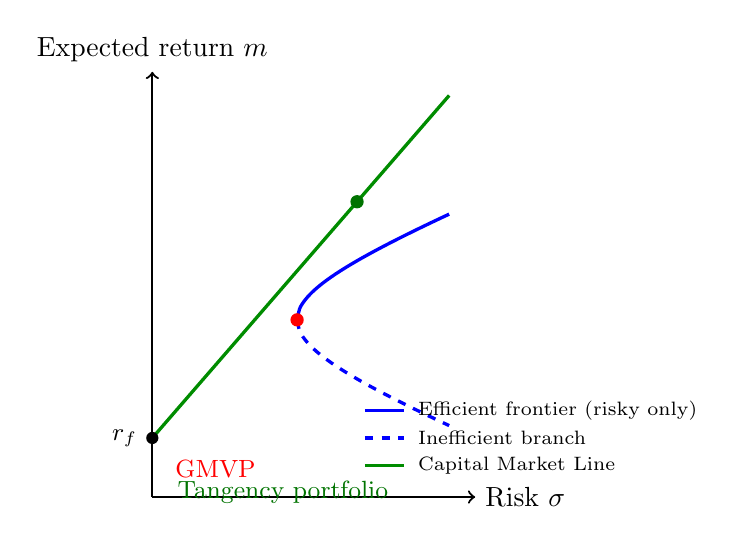
\begin{tikzpicture}[scale=1.0]
% Coordinate model: data (sigma, m) mapped with xscale 2.6, yscale 1.5.
% Parameters: A/C = 1 (GMVP return), 1/C = 0.5 (GMVP variance => sigma_g = 0.7071),
% D/C^2 = 0.5 so that m = 1 +- 0.5*sqrt( (sigma^2 - 0.5)/0.5 ).
\def\xs{2.6} % x scale (per unit sigma)
\def\ys{1.5} % y scale (per unit m)
\def\xo{0}   % origin x in data
\def\yo{-0.5}% origin y in data (so axis starts a bit below rf)

% --- Axes ---
\draw[->, thick] (0,0) -- (4.1,0) node[right] {Risk $\sigma$};
\draw[->, thick] (0,0) -- (0,5.4) node[above] {Expected return $m$};

% --- Efficient frontier (upper branch), solid blue ---
\draw[blue, very thick, domain=0.7072:1.45, smooth, variable=\s, samples=60]
  plot ({(\s-\xo)*\xs}, {((1 + 0.5*sqrt((\s*\s - 0.5)/0.5)) - \yo)*\ys});

% --- Inefficient frontier (lower branch), dashed blue ---
\draw[blue, very thick, dashed, domain=0.7072:1.45, smooth, variable=\s, samples=60]
  plot ({(\s-\xo)*\xs}, {((1 - 0.5*sqrt((\s*\s - 0.5)/0.5)) - \yo)*\ys});

% --- Capital Market Line: m = r_f + slope*sigma, r_f = 0, slope chosen for tangency look ---
\draw[green!55!black, very thick]
  ({(0-\xo)*\xs},{(0-\yo)*\ys}) -- ({(1.45-\xo)*\xs},{(0 + 2.0*1.45 - \yo)*\ys});

% --- GMVP point ---
\fill[red] ({(0.7072-\xo)*\xs},{(1-\yo)*\ys}) circle (2.4pt);
\node[red, anchor=west] at ({(0.7072-\xo)*\xs+3pt},{(1-\yo)*\ys+8pt}) {\small GMVP};

% --- risk-free point ---
\fill[black] ({(0-\xo)*\xs},{(0-\yo)*\ys}) circle (2.2pt);
\node[anchor=east] at ({(0-\xo)*\xs-2pt},{(0-\yo)*\ys}) {\small $r_f$};

% --- tangency point (approx where CML meets upper hyperbola) ---
\fill[green!45!black] ({(1.0-\xo)*\xs},{(2.0-\yo)*\ys}) circle (2.4pt);
\node[green!45!black, anchor=west] at ({(1.0-\xo)*\xs+3pt},{(2.0-\yo)*\ys-2pt})
   {\small Tangency portfolio};

% --- Legend ---
\begin{scope}[shift={(2.7,0.5)}]
  \draw[blue, very thick] (0,0.6) -- (0.5,0.6);
  \node[anchor=west] at (0.55,0.6) {\scriptsize Efficient frontier (risky only)};
  \draw[blue, very thick, dashed] (0,0.25) -- (0.5,0.25);
  \node[anchor=west] at (0.55,0.25) {\scriptsize Inefficient branch};
  \draw[green!55!black, very thick] (0,-0.1) -- (0.5,-0.1);
  \node[anchor=west] at (0.55,-0.1) {\scriptsize Capital Market Line};
\end{scope}
\end{tikzpicture}
\end{center}

\noindent The blue hyperbola is the minimum-variance frontier of
Theorem~\ref{thm:parabola}; its solid upper branch is efficient. The red dot is
the GMVP (Corollary~\ref{cor:gmvp}). When a risk-free asset is added, the
efficient set becomes the green Capital Market Line, tangent to the hyperbola at
the tangency portfolio (Theorem~\ref{thm:onefund}).

\section*{Summary of Key Quantities}
\addcontentsline{toc}{section}{Summary of Key Quantities}

\begin{center}
\renewcommand{\arraystretch}{1.5}
\begin{tabular}{ll}
\hline
Quantity & Expression \\
\hline
Scalars & $A = \one\T\bSigma^{-1}\bmu$, \;
           $B = \bmu\T\bSigma^{-1}\bmu$, \;
           $C = \one\T\bSigma^{-1}\one$, \;
           $D = BC - A^2$ \\
Frontier portfolio & $\bw^\star(m) = \dfrac{Cm-A}{D}\bSigma^{-1}\bmu
                       + \dfrac{B-Am}{D}\bSigma^{-1}\one$ \\
Frontier variance & $\sigma^2(m) = \dfrac{Cm^2 - 2Am + B}{D}$ \\
GMVP & $\bw_{\mathrm{g}} = \dfrac{1}{C}\bSigma^{-1}\one$, \;
       $m_{\mathrm{g}} = A/C$, \; $\sigma_{\mathrm{g}}^2 = 1/C$ \\
Tangency & $\bw_{\mathrm{T}} = \dfrac{\bSigma^{-1}(\bmu - r_f\one)}{A - Cr_f}$ \\
Max Sharpe ratio & $\sqrt{(\bmu - r_f\one)\T\bSigma^{-1}(\bmu - r_f\one)}$ \\
\hline
\end{tabular}
\end{center}

\end{document}
